\section{Anforderungen an externe Schnittstellen}
\subsection{Benutzeroberflächen}
% 3.1 und 3.4 überschneiden sich. 
% 3.4 eher über Rechnergrenzen und 3.1 nur lokal
% haben wir aber schon richtig gemcht
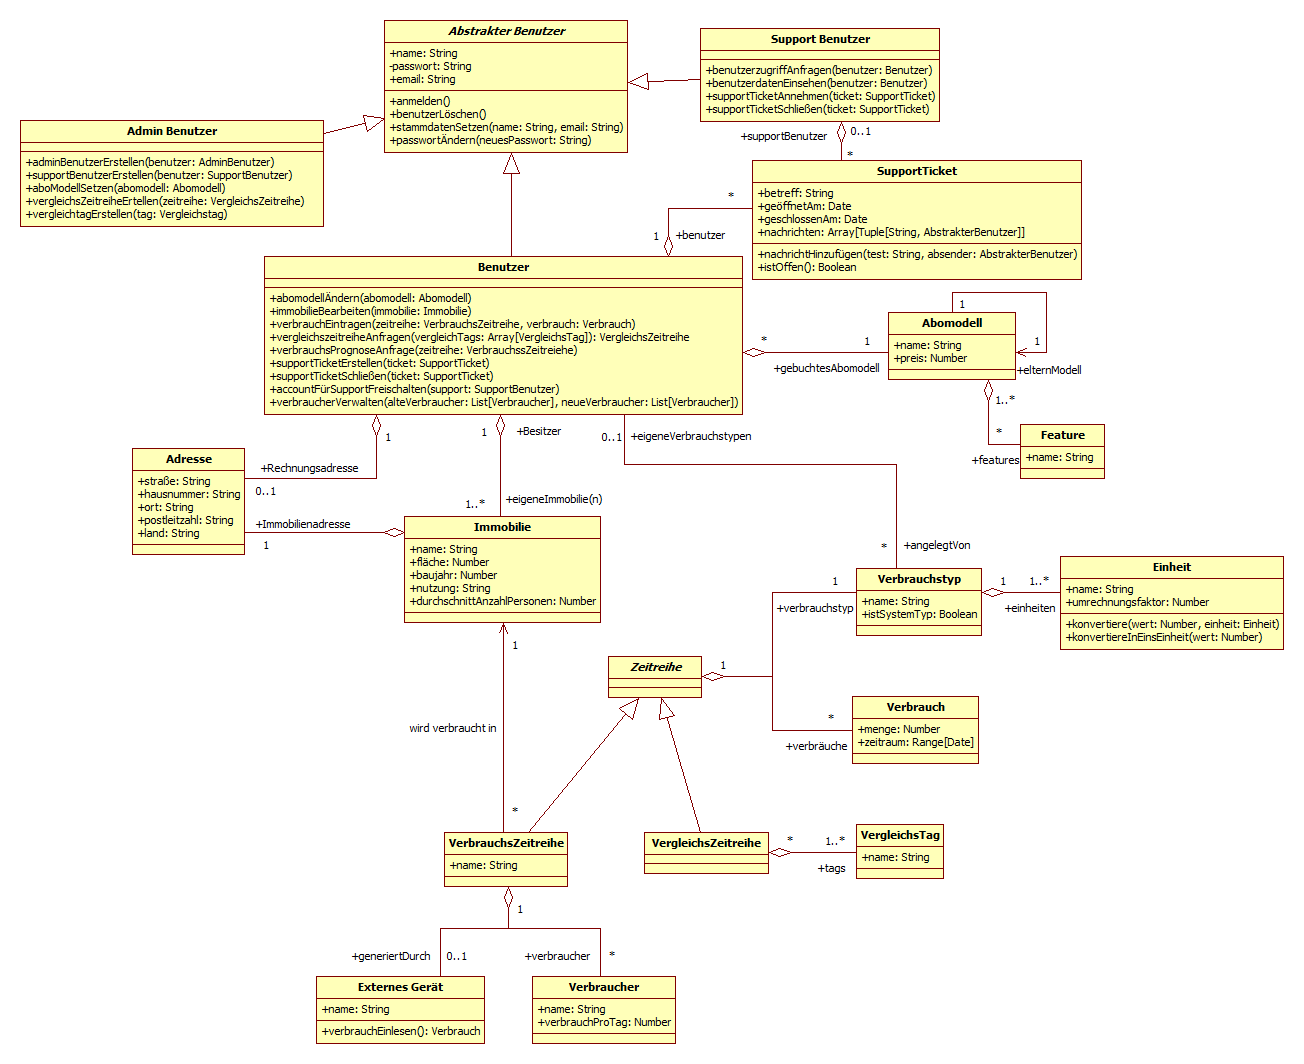
\includegraphics[scale=0.3]{klassendiagramm.png}
\subsubsection{Benutzeroberfläche}
Die Software bietet ein User-Interface welches Zugriff auf alle Standard Funktionen, wie Verbrauch eintragen, Verbrauch vergleichen oder Statistiken anzeigen bereitstellt.
\subsubsection{Supportoberfläche}
Über ein Support Interface soll erweiterter Zugriff auf User Accounts nach deren Freigabe möglich sein.
\subsubsection{Adminoberfläche}
Es wird ein Admin Interface bereitgestellt, welches vollkommene Kontrolle über alle Funktionalitäten hat.
Insbesondere soll es möglioch sein, Vergleichszeitreihen anzulegen und die Funktionalitäten, die den Abo-Modelln zugeordnet sind, anzupassen.
\subsection{Hardware-Schnittstellen}
Die Software bedient sich keiner Hardware Interfaces.
\subsection{Software-Schnittstellen}
\subsubsection{Stadtwerke}
Die Software bezieht, sofern vorhanden, Daten aus den örtlichen Stadtwerken um Statistiken bereitzustellen mit denen der eigene Verbrauch verglichen werden kann.
\subsubsection{Zahlungsdienstleister}
Ein Austausch mit den Zahlungsdienstleistern ist erforderlich um Zahlungen für Premium Versionen gewährleisten zu können.
\subsection{Kommunikationsschnittstellen}
Die Kommunikation der Einzelnen Interfaces erfolgt über HTTPS.